\documentclass[10pt,twocolumn,letterpaper]{article}

\usepackage{cvpr}
\usepackage{times}
\usepackage{epsfig}
\usepackage{graphicx}
\usepackage{amsmath}
\usepackage{amssymb}
\usepackage{soul}

% Include other packages here, before hyperref.

% If you comment hyperref and then uncomment it, you should delete
% egpaper.aux before re-running latex.  (Or just hit 'q' on the first latex
% run, let it finish, and you should be clear).
\usepackage[pagebackref=true,breaklinks=true,letterpaper=true,colorlinks,bookmarks=false]{hyperref}

\cvprfinalcopy % *** Uncomment this line for the final submission

\def\cvprPaperID{****} % *** Enter the CVPR Paper ID here
\def\httilde{\mbox{\tt\raisebox{-.5ex}{\symbol{126}}}}

% Pages are numbered in submission mode, and unnumbered in camera-ready
\ifcvprfinal\pagestyle{empty}\fi
\begin{document}

%%%%%%%%% TITLE
\title{Fast Cross-Domain Unsupervised Object detection through Online Domain Transfer}


\author{Guido Ricioppo\\
Politecnico di Torino\\
Turin, Italy\\
{\tt\small s279127@studenti.polito.it}
% For a paper whose authors are all at the same institution,
% omit the following lines up until the closing ``}''.
% Additional authors and addresses can be added with ``\and'',
% just like the second author.
% To save space, use either the email address or home page, not both
\and
Mazin Onsa\\
Politecnico di Torino\\
Turin, Italy\\
{\tt\small s252865@studenti.polito.it}
\and
Thomas Constantin \\
Politecnico di Torino \\
Turin, Italy \\
{\tt\small s265651@studenti.polito.it}}

\maketitle
%\thispagestyle{empty}

%%%%%%%%% ABSTRACT
\begin{abstract}
    The problem of detecting objects in various image domains without high availability of annotations is still an novel task. The most promising works which addresses the problem reached interesting results relying on image level annotation in a target domain. However the existing frameworks requires time consuming fine-tuning processes of a fully supervised object detector. Furthermore the slow process of domain translation from a source to a target domain severely limits the variability of target image domains. In this paper, we present a framework for cross-domain unsupervised object detection exploiting real-time domain adaptation. We start from a fully supervised object detector trained on a source domain (e.g., natural image) composed of instance-level annotated images and progressively adapt the detector using unsupervised images from a target domain (e.g., artwork). Our framework performs fine-tuning without previously translated samples, achieving a fast and versatile domain adaptation. We also improve the mean average precision (mAP) compared to other domain translation methods.
\end{abstract}

%%%%%%%%% BODY TEXT

\section{Introduction}

Machine learning, particularly with the Deep Convolutional Neural Network (DNNs), has achieved great success in the task of object instance detection and its classification, even with multiple objects in a single image. This success faces the challenge of detecting images on different visual domains.   
%%Addressing the problem of UDA in OD
Domain adaptation (DA) refers to the goal of learning a concept from labeled data in a source domain that performs well on a different but related target domain \cite{ganin2016domainadversarial, Goodfellow-et-al-2016, 5288526}. Unsupervised domain adaptation (UDA) specifically addresses the situation where there are labeled source data and only unlabeled target data available for use during training \cite{ganin2016domainadversarial, long2015learning}. Specifically when we address the problem of object detection, labels refer to annotations i.e. object class labels and corresponding bounding boxes, and learning refers to the process of re-adjusting the parameters of the DNN that performs the object detection 

\begin{figure}[t]
\begin{center}
\fbox{
   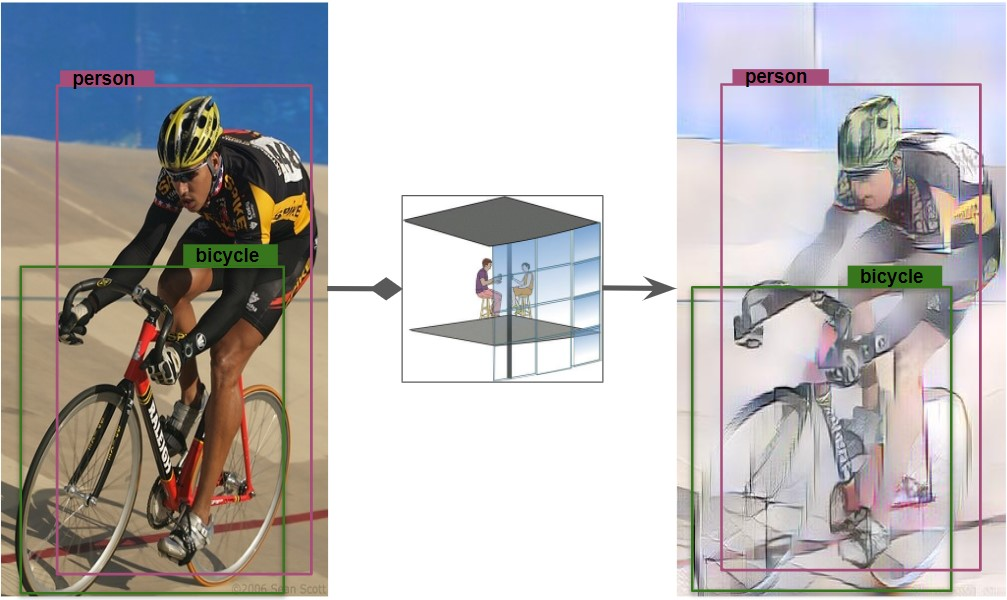
\includegraphics[width=0.96\linewidth]{Images/Domain Transfer1.jpg}}
\end{center}
   \caption{Example of domain transfer used in our method. The style translated image was originally on the source domain, hence it is instance-level annotated. }
\label{fig:long}
\label{fig:onecol}
\end{figure}

Because of its ability to adapt labeled data for use in a new application, DA can reduce reliance on potentially-costly target data labels. As an example, consider the current challenge of object detection in autonomous vehicles. Different weather,road and traffic conditions,  produces many visual domains to be considered for the task \cite{shan2019pixel} and since manual annotation task is very costly, human annotation could be spared by training an object detection model on synthetic images (the source domain) since these can be cheaply generated, then adapting and testing for real street view images (the target domain).
%% attempts of UDA in different fields + downsides
%% 1- domain invariant
Based on the theory of {\it Ben-David et al.} \cite{36364}, the majority of recent DA works \cite{long2018conditional} lay emphasis on how to minimize the domain divergence. Most methods align source and target domains by creating a domain-invariant feature representation \cite{bousmalis2017using, 36364, 8578386}, typically in the form of a feature extractor neural network. A feature representation is domain-invariant if the features follow the same distribution regardless of whether the input data are from the source or target domain \cite{zhao2019learning}.

Alignment can be achieved by minimizing divergence \cite{gretton2008kernel, JMLR:v13:gretton12a}, performing reconstruction \cite{ghifary2016deep}, and some employ adversarial training commonly using generative adversarial networks (GANs) \cite{ganin2016domainadversarial, ganin2015unsupervised}.However, these methods assume that such a feature representation exists and the marginal label distributions do not differ significantly.


%% 2- domain mapping with emphasize on conditional gans since it's our competetor in synthetic generation
An alternative to creating a domain-invariant feature representation is mapping from one domain to another most commonly by image-to-image translation (I2I) aiming to make images indistinguishable across domains \cite{choi2018stargan,lee2018diverse,liu2018unsupervised,CGAN}. The mapping is typically created adversarially and at the pixel level.

This mapping can be accomplished with a conditional GAN. The generator performs adaptation at the pixel level by translating a source input image to an image that closely resembles the target distribution \cite{denton2015deep, goodfellow2014generative, mirza2014conditional} conditioning on an input image. A typical configuration as shown in Figure \ref{fig:ConditionalGAN} mapping an input image from one domain (e.g. realistic) to an output image in another domain (e.g. synthetic). 

The major downside of the increasingly widespread use of adversarial techniques in DA is the high computational cost: while conditional GAN well performed for classification and detection for UDA, good results comes at long training times. For example as per \cite{pasqualino2020unsupervised}, it took 66 days for faster RCNN pretrained on "EGO-CH" dataset to adapt on a 16 object artwork dataset using a single and CycleGAN for the Domain Transfer as shown in figure \ref{fig:cost}. Generally, recent GANs are 1-2 orders of magnitude more computationally intensive than modern recognition CNNs. Very recent attempts such as \cite{li2020gan} tried to increase the performance using compression techniques.
%% our contributaion

We propose a new and faster UDA framework for the object detection task by utilizing a real-time I2I translation network extracts the style feature of the image to generate a target-like images. 

Unlike other domain mapping synthetic images generators, this style transfer network - based on the normalization statistics - has a simple architecture, parameter free and synthetic images will be generated {\it online}, as shown in Figure \ref{fig:long}, to guarantee fast adaptation for the OD.


\begin{figure} [b]
   \centering
   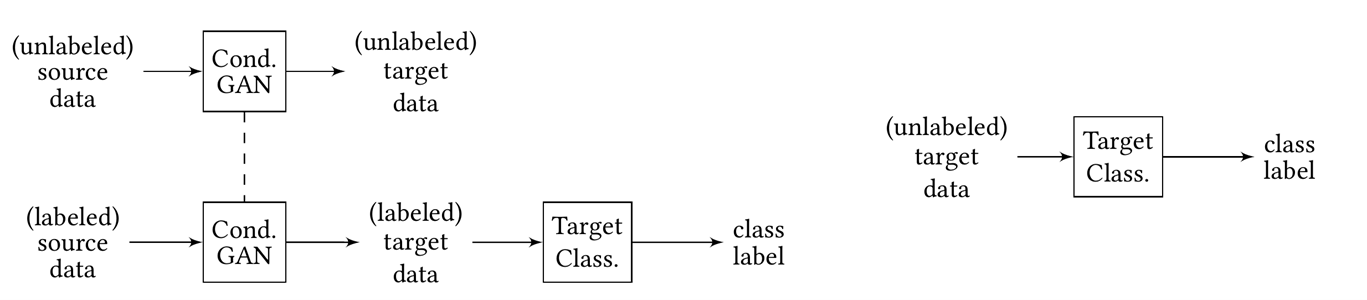
\includegraphics[width=0.48\textwidth]{Images/conditionalgan_syn_generation.png}
   \caption{conditional GAN configuration for UDA}
\label{fig:ConditionalGAN}
\end{figure}

Our main contributions summary is:
\begin{itemize}
    \item the proposed framework leverages the accuracy of the baseline FSD by approximately 10 to 12 percentage points in terms of mAP
    
    \vspace{15mm}
    \item In comparison against the best performing unsupervised domain mapping algorithms in the cross domain adaptive detection, our framework outperforms these algorithms by 4 to 5 percentage points.
    \item In addition to the best performances related to mAP, we stated a relevant reduction in terms of DT time.
\end{itemize}

The code of our project is available at \url{ https://github.com/guidonguido/DA_detection}



%-------------------------------------------------------------------------



\begin{figure}
\begin{center}
%\fbox{\rule{0pt}{2in} \rule{.9\textwidth}{0pt}}
   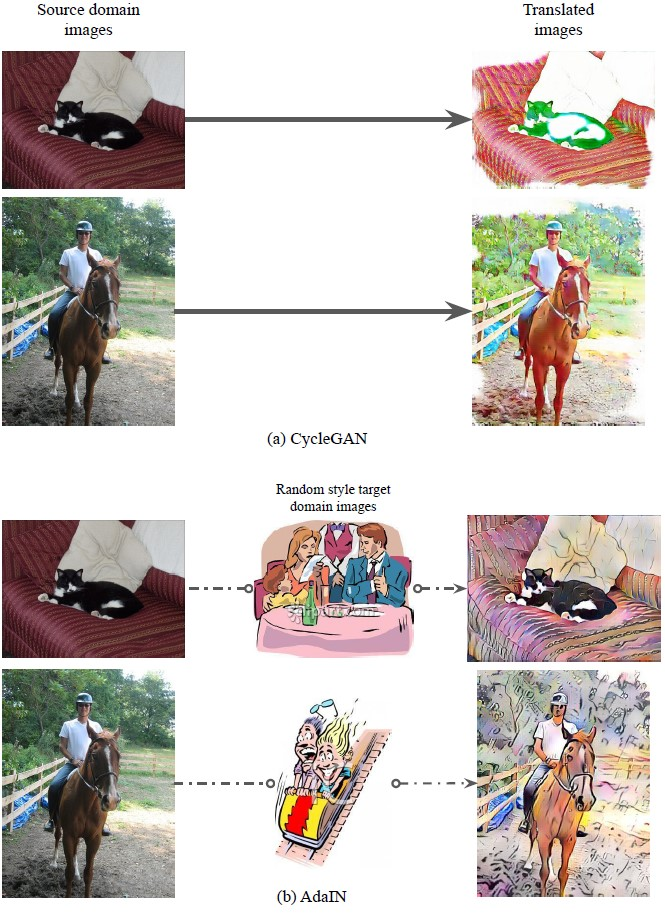
\includegraphics[width=0.48\textwidth]{Images/Translation2.jpg}
\end{center}
   \caption{Example of image translation obtained with two techniques. CycleGAN (a) is trained to learn the mapping function between the source domain and the target domain. For AdaIN (b) a generic pre-trained model is needed.}
\label{fig:Translation}
\end{figure}

%------------------------------------------------------------------------
\section{Related Work}
%OD
%UDA+UDA for OD
%i2i translation
%style transfer
%i2i for UDA+for UDA for OD
%------------------------------------------------------------------------
\subsection{Object Detection}
Object detection is a task to locate and classify objects in an image or video. Starting from 2013, Convolutional neural networks (CNNs) had a huge impact on the raise of the mean Average Precision (mAP) that passed from \(40.6\textit{\%}\) in 2012 \cite{shallowOD} to \(74.9\textit{\%}\) with SSD \cite{SSD} on the same VOC 2007 and VOC 2012 datasets \cite{VOC}.

Object detection can be achieved using different techniques: {\it sliding window} applies a CNN to many portions of the image, classifying each portion as object or background. 
R-CNN and its variations \cite{R-CNN, FastR-CNN, FasterR-CNN} ease the computation complexity implementing {\it region proposals}. Different regions of interest (RoI) are proposed and each region is forwarded toward a CNN, calculating and refining a multi-task loss composed by classification and bounding-box regression loss.
These models are called two-stage detectors and reach the highest accuracy rates, but they are typically slower.

The second state-of-the-art object detectors known as the single-stage detectors such as YOLO and SSD \cite{Yolov2, SSD} implement {\it detection without proposal}: first a  fixed-size collection of bounding boxes are generated, each box produces a score for the presence of objects and finally a intersection over union (IoU) threshold is used to produce the final decision. This technique can choose between boxes with different scales and aspect ratios, so this technique is effective with instances with different positions and distance from the camera.
Original SSD architecture is based on a VGG16 \cite{vgg} backbone and an extra feature layer box-head.
Such models reach lower accuracy rates but are much faster than two-stage object detectors.

 We use SSD as an object detector – without loss of generality - for its fast performance, competitive accuracy results specially on larger objects and to guarantee fair comparison since it is the same baseline used in \cite{CrossDomObjDet}
%---------------------------------------------------------------

\subsection{Unsupervised Domain Adaptation}
%%addressing the need DA for OD 
Fully supervised object detectors (FSD) \cite{R-CNN, FastR-CNN, FasterR-CNN, Yolov2, SSD} perform outstandingly when natural image domains datasets are available with instance-level annotations. These same models, however, record a not negligible decrease in the performance when the target domain is different from the training one, as shown in \cite{BAM} and \cite{CrossDomObjDet}.

%% the challenge of annotation
The construction of a new dataset with instance-level annotations is a heavy and time-consuming task, since it requires the manual definition of (potentially) multiple ground truth boxes for each image.

Given a source domain \(\mathit{D^s}\) characterized by a feature space \(\mathit{X}\) and a target domain \(\mathit{D^t}\) with a feature space \(\mathit{Y}\), in supervised DA every target data in \(\mathit{D^t}\) has instance-level annotations.


%------------------------------------------------------------------------
%I2I translation originally implemented without DA
\subsection{I2I Translation}

A popular and general-purpose supervised method is pix2pix, developed by {\it Isola et al.} \cite{isola2018imagetoimage}. Based on pix2pix, comes the most recently used technique CycleGAN \cite{CGAN}.This approach is capable of learning to translate an image from \(\mathit{D^s}\) to \(\mathit{D^t}\) while input-output examples are unpaired (UI2I). However, the generation of new images cannot be achieved in real-time, during the fine-tuning process. It requires a CycleGAN training phase, where the model learns how to generate effective translated images. Training the model is a heavy process and very time-consuming, even with modern GPUs. 
As we did in our work, training the CycleGAN for 20 epochs using the default configurations and a machine with 12GB RAM, Tesla T4 6 GB GDDR6 will take up to 3 days.

The translated images in \cite{CGAN} provide outstanding results with 200 epoch training. In Figure \ref{fig:Translation} (a) it is shown an example of CycleGAN translation.

\subsection{Progressive Domain Adaptation}
%% TODO: Cyclegan and othe DA methods
%%      Aggiungi immagini di esempio da due domini diversi

These {\it I2I} translation approaches map images from one domain to another without the explicit purpose of performing domain adaptation, they can also be used for domain adaptation. For example, the original CycleGAN paper was application agnostic, but others have experimented with applying CycleGAN to domain adaptation \cite{benaim2017onesided,fu2018geometryconsistent,hoffman2017cycada}. It is important to note though that these image-to-image translation approaches assume that the domain differences are primarily low-level \cite{bousmalis2017unsupervised,bousmalis2017using,tzeng2017adversarial}.

Our work followed the path traced in \cite{CrossDomObjDet}, where a fully supervised detector (FSD) is trained on \(\mathit{D^s}\) and then {\it fine-tuned} on \(\mathit{D^t}\). Since there are no instance-level annotations in \(\mathit{D^t}\), the progressive domain adaptation is obtained by {\it domain transfer} (DT). 

DT can be obtained by artificially and automatically translating the appearance of  \(\mathit{D^s}\) images such that they look like those in the target domain. In that way new \(\mathit{D^t}\) images with instance-level annotation are used for the fine-tuning phase.



%------------------------------------------------------------------------



\subsection{Style Transfer}
Style transfer aims at altering the low-level visual style within an image while preserving its high-level semantic content. {\it Gatys et al.} \cite{cordts2016cityscapes} proposed the seminal idea to combine content loss and style loss based on the pre-trained neural networks on ImageNet \cite{chen2018domain}. Based on this pioneering work, {\it Huang et al}. \cite{goodfellow2014generative} proposed the AdaIN to match the mean and variance statistics of the latent embedding of the content image and style image, then decoded the normalized feature into a stylized image. We used the latter technique to achieve DT; an exaple of generated images is shown in Figure \ref{fig:Translation} (b).

Another line of works \cite{li2018semanticaware,zheng2020rectifying,huang2018multimodal} is based on the generative adversarial network (GAN) \cite{goodfellow2014generative}, which employs a discriminator to supervise the style transfer. 
%------------------------------------------------------------------------

\begin{figure*}
\begin{center}
%\fbox{\rule{0pt}{2in} \rule{.9\textwidth}{0pt}}
   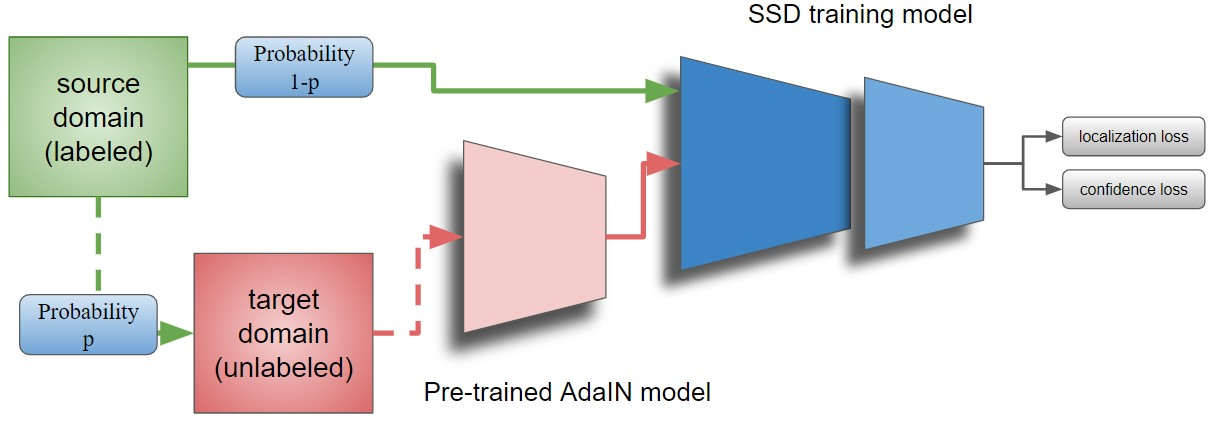
\includegraphics[width=1\linewidth]{Images/variation_architecture.jpg}
\end{center}
   \caption{The framework developed for our method. The likelihood {\it p} is set to \(0\) during the pre-training of SSD300, while it will have a value \( (0,1]\) to fine-tune the detector.}
\label{fig:Architecture}
\end{figure*}


%------------------------------------------------------------------------
\section{Proposed Method}
We propose a real-time domain translation from labeled source image dataset (realistic) to unlabeled target dataset (artistic) to adapt a FSD pretrained on the source domain. The adaptation is achieved through fine-tuning of the FSD on artificially generated samples with instance-level annotations using the style of images in the target domain to translate those on source domain.

First, we pre-train the FSD using instance-level annotated images from the source domain, then we fine-tune it while using images obtained by translating the style of source images to match the target ones.

%%Figure to show the workflow of proposed method
\subsection{Online Style Transfer}
Normalization techniques such as Batch normalization and Instance normalization have been used for a while in DNN, however, none of these normalization techniques were developed with domain translation in mind. 

We will exploit the AdaIN framework \cite{AdaIN} for cross-domain bject detection.

Due to the differences between the source and target domains, in order to improve mAP of the object detector on target images, we applied a real-time style transfer technique to generate images that look like those in the target domain.

The AdaIN framework receives a content input \(x\) and a style input \(y\), and simply aligns the channel-wise mean and variance of \(x\) to match those of \(y\); It computes the affine parameters from the style input:


\[ AdaIN(x)=\sigma(y)\left(\ \frac{x-\mu(y)}{\sigma(x)} \right)\ +\mu(y) \]

where \(\mathit{{\mu(x),\sigma(x)}}\) are the mean and standard deviation of the input images. The normalized content input is scaled with \(\mathit{\sigma(x)}\) and shifted with \(\mathit{\mu(y)}\). These statistics are computed across spatial locations.


In order to have a comparison with existing models [References to other models], we evaluated the model using different likelihood to quantify the detection improvements AdaIN transformation had on the base model. A random image taken from the clipart dataset was used as style input. The logical framework used in our experiments is shown on Figure \ref{fig:Architecture}.


%------------------------------------------------------------------------
\section{Dataset}
The first step of our work is meant to train the model using the source domain dataset \(\mathit{D^s}\). Since the fine-tuning phase will exploit the knowledge acquired during the first training, it is necessary that the target domain \(\mathit{D^t}\) classes are all or a subset of the classes in \(\mathit{D^s}\).

During the first training phase we used PASCAL VOC \cite{VOC}, composed by real images not filtered for "quality" which means the objects are in sundry scenes, scale, position, lighting.
VOC consists of 20 classes, and each image is provided with a corresponding instance-level annotation.

On the fine-tuning phase Clipart1k \cite{CrossDomObjDet} was used in order to achieve domain translation. The target domain is used during the CycleGAN \cite{CGAN} training phase, as well as style dataset used by AdaIN \cite{AdaIN} for the domain translation.
Clipart1k is composed by 1,000 images and the same 20 classes present in VOC.

While Clipart1k was designed to perform self-supervised tasks, we never used the image level annotations, since we aim to perform cross-domain unsupervised object detection. 

%------------------------------------------------------------------------
\section{Experiments}
To evaluate the performance of our work, we used mean average precision (mAP), following the experimental methods in \cite{CrossDomObjDet}, which we compare to.  


\begin{table*}
\caption{Comparison of our method and other UDT in terms of AP[\%]. {\it Compared} and {\it proposed} refers to 20,000 fine-tuning iterations starting from SSD300 (60k iterations) as the baseline FSD. \label{table:tableResults}}
\begin{center}
\resizebox{\linewidth}{!}{\begin{tabular}{cllllllllllllllllllllc}

\multicolumn{20}{c}{AP for each class} \\
\cline{2-21}
 Method & aero & bike & bird & boat & bottle & bus & car & cat & chair & cow & table & dog & horse & mbike & person & plant & sheep & sofa & train & tv & mAP \\
 
\hline
{\it Baseline} \\

60k iter & 23.8 & 59.5 & 18.3 & 15.2 & 7.6 & 56.8 & 35.0 & 5.0 & 43.2 & 12.1 & 31.5 & 13.1 & 31.0 & 48.3 & 42.2 & 24.3 & 3.60 & 28.8 & 19.5 & 26.6 & 27.3 \\

120k iter & 21.5 & 46.4 & 18.8 & 11.51& 15.8 & 34.9 & 31.3 & 5.7 & 41.3& 10.4 & 28.0 & 10.0 & 22.3 & 48.0 & 33.8 & 26.8 & 4.4 & 24.6 & 21.3 & 17.1 & 23.7 \\

\hline
{\it Compared} \\

UDT & 22.1 & 61.5 & 20.2 & 18.6 & 21.1 & 61.3 & 42.7 & 6.0 & 44.6 & 31.0 & 32.7 & 11.2 & 28.8 & 57.0 & 51.8 & 36.3 & 20.2 & 26.9 & 32.5 & 38.5 & 33.25\\

\hline
{\it Proposed} \\

p=0.5 & 28.7 & 62.4 & 26.8 & 27.4 & 25.5 & 64.3 & 48.2 & 7.1 & 46.4 & 49.3 & 41.5 & 16.3 & 36.7 & 62.1 & 57.7 & 37.4 & 15.5 & 28.1 & 34.0 & 42.1 & 37.9 \\

p=1.0 & 29.5 & 60.7 & 25.4 & 28.3 & 25.7 & 70.3 & 50.6 & 11.9 & 46.8 & 51.4 & 42.3 & 17.5 & 34.6 & 66.0 & 60.4 & 38.0 & 17.8 & 30.0 & 39.6 & 45.5 & 39.7 \\


\hline

Ideal case & 50.5 & 60.3 & 40.1 & 55.9 & 34.8 & 79.7 & 61.9 & 13.5 & 56.2 & 76.1 & 57.7 & 36.8 & 63.5 & 92.3 & 76.2 & 49.8 & 40.2 & 28.1 & 60.3 & 74.4 & 55.4 \\

\hline





\end{tabular}}
\end{center}
\end{table*}

\subsection{Experimental setup}
VOC07-trainval and VOC12-trainval \cite{VOC} were used for the first model training phase and fine-tuning phase. We used this same splits for the CycleGAN \cite{CGAN} train, translating a total of \(16551\) images.

Unlabeled images from Clipart1k \cite{CrossDomObjDet} were used as target-domain images. For the fine-tuning phase we used the train split, which counts 500 images corresponding to half of the entire dataset.

Every test is performed on the remaining 500 images in Clipart1k. Following the analysis pattern in \cite{CrossDomObjDet}, we reproduced the latter results comparing the two methods.


\subsection{Baseline model}
We used SSD300 as baseline model for object detection. Our implementation is based on \cite{lufficc2018ssd} and only slight modifications were made to perform online image to image transformation. Figure \ref{fig:Architecture} shows a logical representation of the used framework. Every analysis parameter and model modification is listed on further sections.

Train images are transformed to \(300 \text{ x } 300\) input size and other transforms were applied with \(50\%\) probability, like mirror and sample crop, in addition to applying some photo-metric distortions \cite{SSD}. The choice to use SSD300 and not SSD512 is due to the fact that we pre-trained the baseline model ourselves, therefore increasing the input size would have caused not negligible increase of training time. Also, using SSD300 as \cite{CrossDomObjDet} did, we can have a better comparison of the results.



\subsection{Pre-training details}
SSD300 was trained during the first phase for 60,000 and 120,000 iterations. During pre-training, batch size is 32 and the learning rate is fixed to \( 10^{-3}\) after an initial warm-up with factor 0.3 every 500 iterations. For that phase VOC07-12 trainval splits were used and the other parameters were the default in \cite{lufficc2018ssd}.

\subsection{Comparison \label{sec:comparison}}
We compare our progressive domain adaptation method against the unsupevised domain transfer method (UDT) proposed in \cite{CrossDomObjDet}. We reproduced the baseline analysis and trained the CycleGAN with VOC07-12 trainval splits as source domain and Clipart1k train split as target domain, with learning rate \(10^{-5}\) for the first ten epochs and a linear epoch decaying rate for the next ten epochs, for a total of 20 epochs. Obtained DT images, we fine-tuned the pre-trained SSD300 for 20,000 iterations with batch size \(1\) and learning rate fixet to \(10^{-6}\).  Ideal case information are also used for comparison: this results were produced accessing to instance-level annotations for the training set of Clipart1k. Results are shown in Table \ref{table:tableResults}.

\subsection{Fine-tuning details}
Fine-tuning was conducted using a pretrained AdaIN \cite{AdaIN} model for 20,000 iterations and batch size 1. We used the architecture showed in Figure \ref{fig:Architecture}: each source domain image (AdaIN content image) is translated in real-time with a probability {\it p}. We evaluated our method with {\it p = 0.5} and {\it p = 1.0}. The parameter {\it alpa}, which controls the fusion degree in AdaIN, was set to 1.

\subsection{Quantitative Results}
Results are shown in Table \ref{table:tableResults}. We compare our method against the baseline FSD and the method mentioned in Sec \ref{sec:comparison} considering the AP for each class and general mAP.

We noticed no increase in terms of mAP doubling the number of iterations during training of the baseline model. On the contrary, 120,000 iterations provides a drop of 3.6 mAP percentage points. Precisely for this reason, all the fine-tuning experiments are executed starting from 60,000 iterations.

\vspace{3mm}

Our method provides an improvement of 10.6 percentage points from the baseline and 4.6 points than the unsupervised domain transfer proposed in \cite{CrossDomObjDet}. 

Both results with 0.5 and 1.0 translation likelihood are still more than 10 percentage points lower the ideal case.

\vspace{3mm}

\textbf{Ablation Study}  We conducted the fine-tuning as proposed in the compared method, after producing the CycleGAN translated images, whit two settings. First time fine-tuning was conducted for 10,000 iterations with batch size 32 and learning rate \(10^{-3}\). Then we fine-tuned the FSD for 20,000 iterations with batch size 1 and learning rate \(10^{-6}\) as explained above. Both times the mAP of the UDT method was approximately 33\%, therefore increasing batch size and consequently training time has no effect on the compared model.

As expected, increasing the style {\it translation probability p} from \(0.5\) to \(1.0\) led to mAP increase. 

\vspace{3mm}

\textbf{Speed Analysis} Results analysis showed the major advantage of our method in terms of fine-tuning time. In Table \ref{table:tableTimes} we compare the speed of our method with the other UDT technique presented in \cite{CrossDomObjDet}. While fine-tuning using online DT images is a fast task, training CycleGAN \cite{CGAN} for 20 epochs took approximately 3 days. Our method uses pretrained AdaIN\cite{AdaIN}: translating each image {\it online} takes 4 seconds at most. Therefore the fine-tuning step is much faster.

\begin{table}
\caption{Speed comparison (in hours). {\it Compared} and {\it proposed} rows refers to fine-tuning 20,000 iterations. \label{table:tableTimes}}
\begin{center}
\begin{tabular}{ccc}
\hline
Method & mAP [\%] & Time (h) \\
\hline
\hline
{\it Baseline} \\
60k iter & 27.3 & 20 \\
120k iter & 23.7 & 40 \\

\hline 
{\it Compared} \\
UDT & 33.25 & 74 \\

\hline
{\it Proposed} \\
p=0.5 & 37.9 & 7.5 \\
p=1.0 & 39.7 & 24 \\

\hline

\end{tabular}
\end{center}
\end{table}



%------------------------------------------------------------------------

\section{Conclusion}

In this paper we proposed a novel solution which improve mAP of FSD in case of domain shift between source images and target ones when instance-level annotations available only in the source dataset.
 %%of this work is the comparison between previous work \ref{} and the CycleGAN and our novel learning method using AdaIN online transformation
Experimental results confirm that adaptive Style transfer not only leverages the accuracy of the UDA of the non trivial task of object detection but also saves high computational cost of the commonly used GANs. 
Our work also proves that a simple architecture, Style-based framework can be used in UDA for OD when a clear domain shift is available. 

\vfill\null
%\cleardoublepage
%------------------------------------------------------------------------
{\small
\bibliographystyle{ieee}
\bibliography{egbib}
}

\appendix
\renewcommand\thefigure{\thesection.\arabic{figure}}    
\section{Figures}
\setcounter{figure}{0}    

\begin{figure}[b]
    \centering
    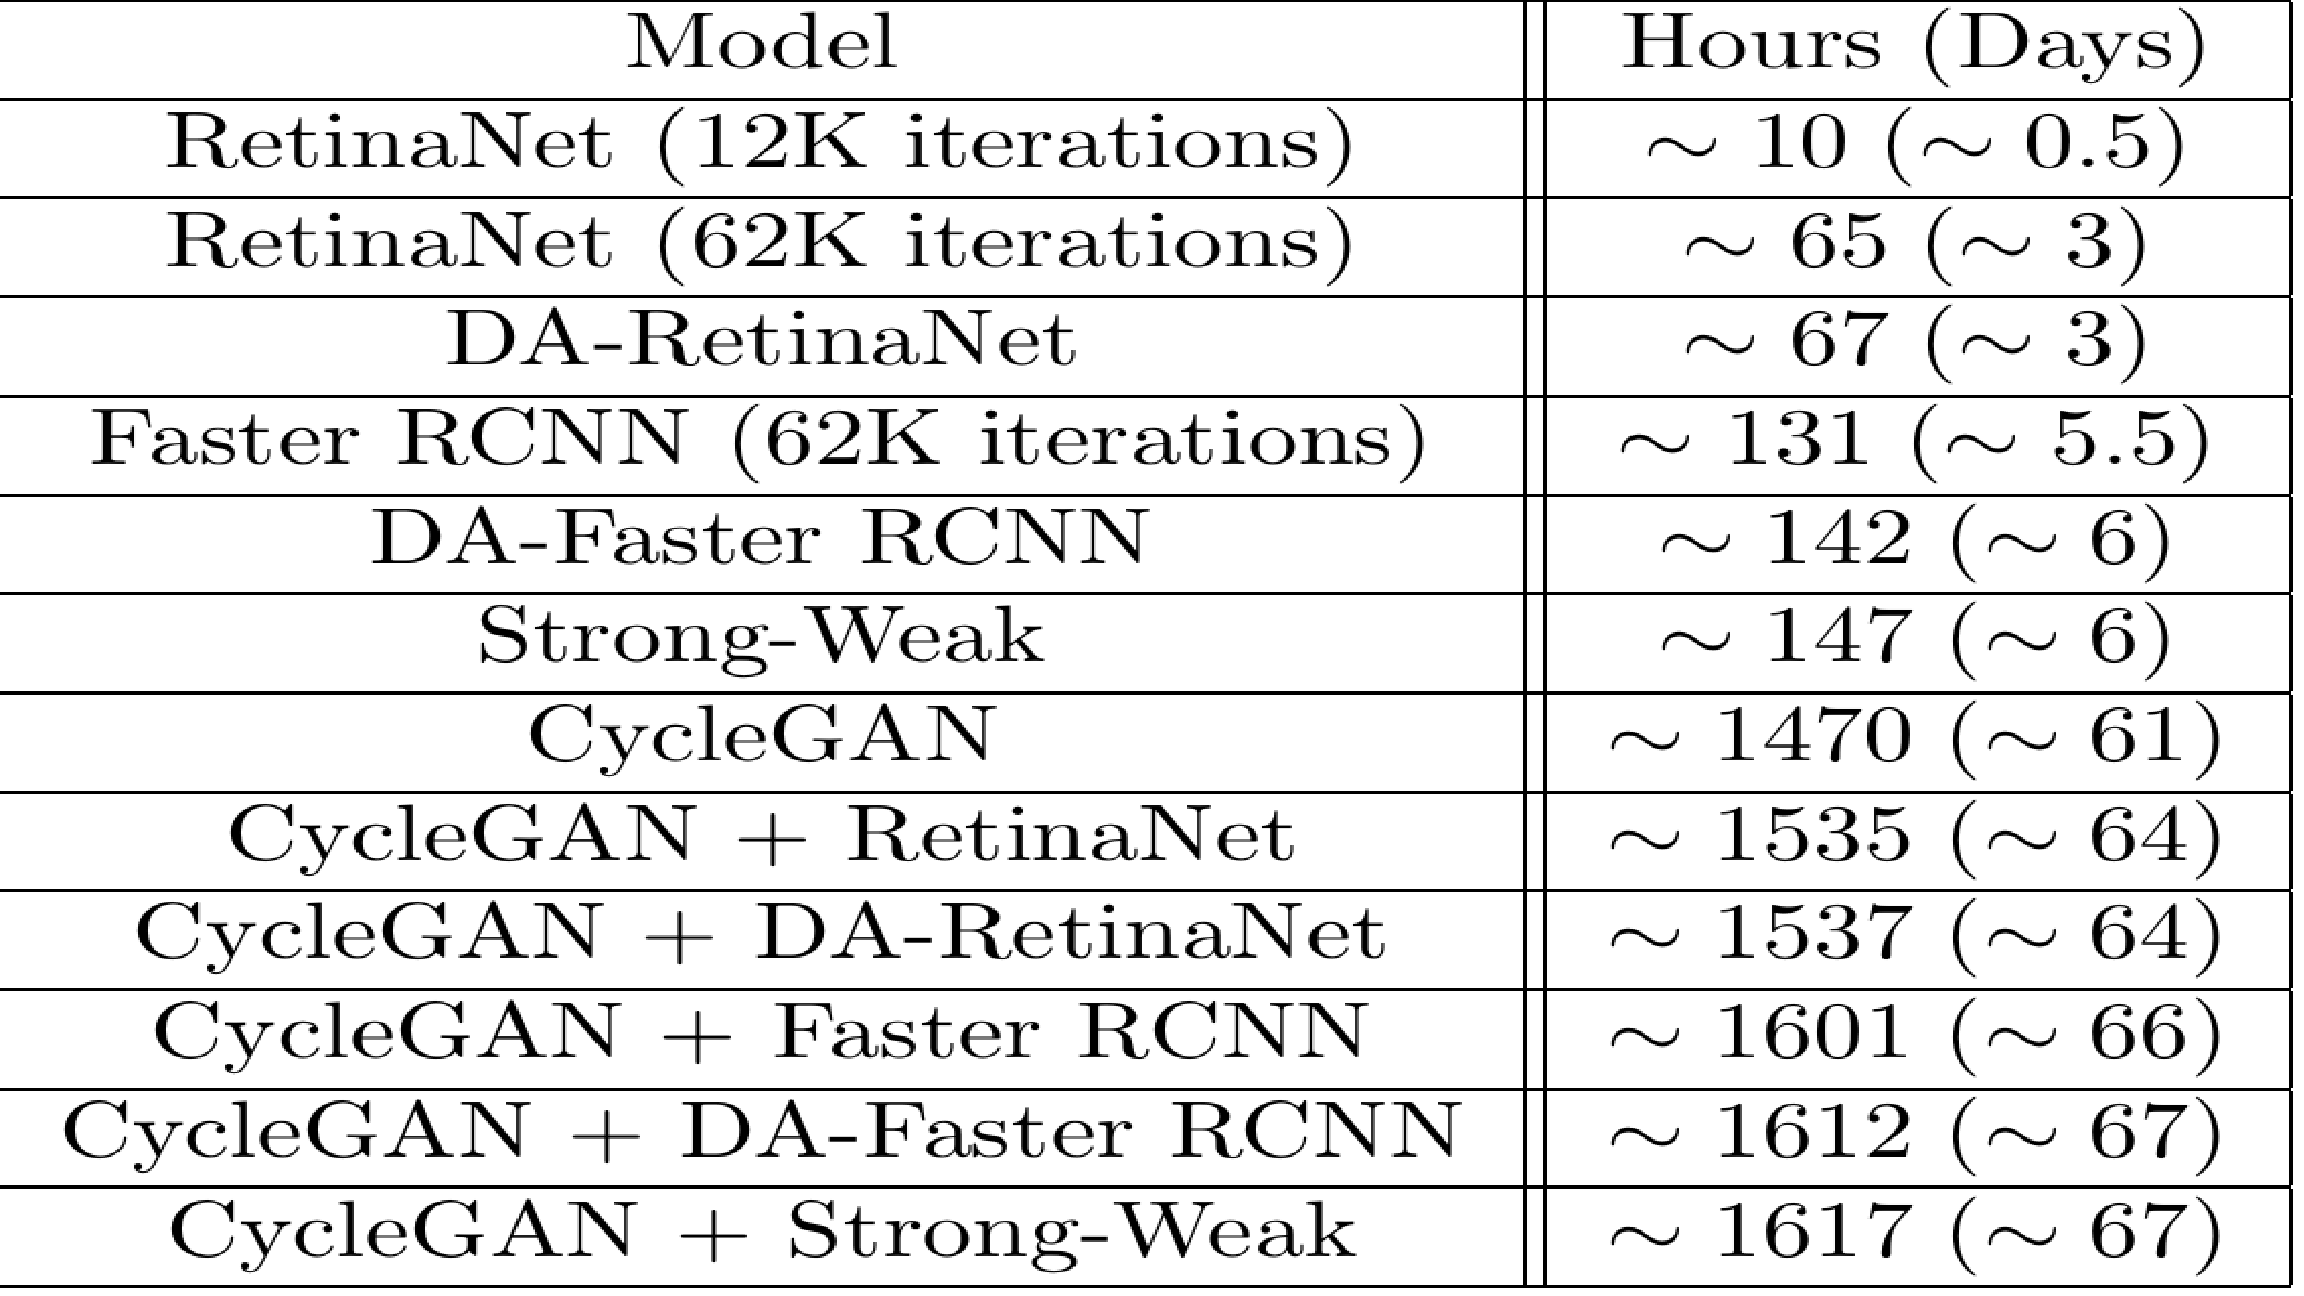
\includegraphics[width=0.96\linewidth]{Images/cyclegan.png}
    \caption{an example of high computational cost of CycleGAN training 60 epochs using the default parameters on a single NVIDIA Tesla K80}
\label{fig:cost}
\end{figure}

\end{document}
